\documentclass[../main/main.tex]{subfiles}

\newdate{date}{15}{04}{2020}

\begin{document}

\section{Lecture 11}
 \displaydate{date}. Compiled:  \today. Martina.

\subsubsection{Slide 179}

\begin{figure}[h!]
\centering
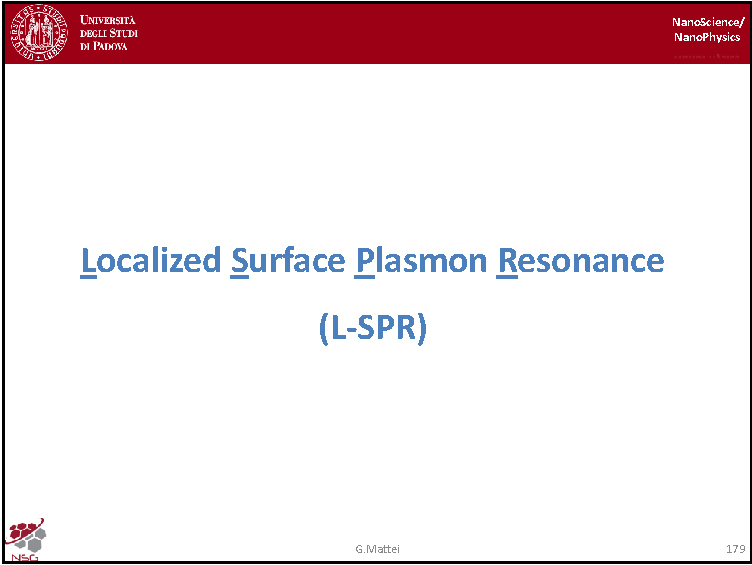
\includegraphics[page=1,width=0.9\textwidth]{../lessons/pdf_file/11_lesson.pdf}
\end{figure}


In the previous lesson we have seen how to experimentally obtain what we called Localized Surface Plasmon Resonance, that is the resonant interaction  between light and matter at the nanoscale, when the material is made out of metallic structure; we have seen how gold nanoparticles with increasing size differ in terms of the intensity of the peculiar resonance in the interaction with monochromatic light as a function of the frequency in the visible range. 

That resonance is called Localized Surface Plasmon Resonance; the word localized will be explained in the following, the concept of resonance is clear and the idea of plasmon is already present in the Solid State Physics course, so you may remember it stands for the collective motion of free electrons in metals and that is a property of that specific metal, as it is related to the square root of the electronic density and to different numeric constants but in principle it is a property of that specific metal. 

In that case we spoke about plasmon resonance in the sense that it is a bulk volume plasmon resonance in the system, that is the whole set of electrons are set in motion with a coherent motion all over the infinite extent of the material;  we will speak about surface plasmon resonance in the sense that is a special kind of plasmonic resonance when you have an interface between two media, that is the metallic structure in form of nanoparticles for instance and the dielectric environment around. The concept of localization of the surface plasmons will be clear in the following.

To extend the description of the basic properties that I would like to discuss with you in this lesson we need to obtain a way to calculate how a plane wave is interacting with our spherical nanostructures. Of course we can attack the problem from a very fundamental point of view that is a quantum mechanic point of view but we will stop very soon because as the number of atoms in the clusters starts to grow, the solution of the complete quantum mechanic Hamiltonian is an untractable problem, so basically there is no perfect solution to this problem.

So instead of a bottom-up quantum mechanic approach we will use a top-down approach in which we will use the classical solution of the problem and we will add quantum mechanic correction to the problem, in what is called semi-classical description of electrons motion in the metallic nanostructures; we will be surprised on how this kind of approach is able to give quantitative results down to very very small nanoparticles, down to a nanometer size, so it's a situation really  similar to the very nice results that we obtained with the classical thermodynamic description of tiny nanoparticles.

\newpage

\subsubsection{Slide 180}

\begin{figure}[h!]
\centering
\includegraphics[page=2,width=0.9\textwidth]{../lessons/pdf_file/11_lesson.pdf}
\end{figure}

So to this aim of course we will start with the electromagnetic description of matter given by Maxwell, and of course we have here the set of Maxwell equations relating electric and magnetic parts of the vectors that we can define to describe all the properties; we need to remember the constitutive equations relating $E$ to $B$, $B$ to $H$ and so on, $\rho_F$ and $j_F$ are the density of free charges and the current of free charges in our material and so on.

What is relevant for us is: can we find a solution of those equations for our problem? That is an incoming plane wave interacting with the spherical isolated nanoparticles in the dielectric. The answer is: yes we can resolve those equations in that particular situation and the solution was given by Gustave Mie in 1908 and the solution was exact in the sense that we have an analytic solution to those equations as a function of the multipolarity of the spherical expansion of the potential as we will see, so this was really a breakthrough in the problem of spherical particles interaction with light which open the field of plasmonics and nanophotonics for metallic mterials. 

The theory of Gustave Mie was not restricted to metals but it holds for any kind of materials in form of nanoparticles, there is no restriction on the size and the only assumption is spherical geometry and the fact that the particle is not embedded in an absorbing medium, which is reasonable assumption and is verified normally in our situation. It was really a very complicated solution, we will see just a very simplified approach just to have a hint of what is going on, and by the way the Mie theory will be able to answer the question: how can we control the colour of a nanoparticle? and we will understand that the question is imposed in the sense that we cannot speak of the colour of that specific particle in a sense that will be clear in the following.

\newpage

\subsubsection{Slide 181}

\begin{figure}[h!]
\centering
\includegraphics[page=3,width=0.9\textwidth]{../lessons/pdf_file/11_lesson.pdf}
\end{figure}

So let's try to enter this problem. Of course in terms of surface plasmon resonance there are  other kinds of surface plasmon resonance and we will be interested in the localized version of that, that is the spr given by a spherical nanoparticle, but there are other kinds of spr, in particular the extended version of that, and i will briefly touch this topic just to give some hint but i will not enter the details, i will just briefly touch it because it is a sort of conceptual state between the full volume surface plasmon resonance and the localized surface plasmons.

The extended spr occurs when we have metal dielectric interface , that is we have our space divided by two semispaces by a planar interface in which we have the separation between a medium with dielectric function $\epsilon_m$ and the metallic structure with dielectric function $\epsilon$. Both are in general complex function of the frequency and in the case of planar interface these solution of Maxwell equations are able to show that you can sustain travelling solution in the plane of the interface with intensity which is an exponentially decreasing function in the normal coordinates whit respect to the surface like in this graph here and we could demonstrate that the condition to achieve the extended spr condition is included in the equation here that is the real part of the dielectric function of the metal should be equal to minus the dielectric function of the medium assuming that the medium is not absorbing; so you may remember this is a generalization of the condition to excite volume plasmon resonance which is $\epsilon_1=0$ and in that case the volume property is a bulk property, a property of that specific material.

In this case you clearly see that the frequency at which we can solve this equation, which is by the way this one if we assume that for the metal we can consider a Drude-like dielectric function, you can clearly see that this is not an intrinsic property of the metal but it depends on the coupling between the metal and the dielectric, and this is an interesting result that we will further comment in the following, in particular in the case of localized nanoparticles. 

This kind of modes, even if the solution of the Maxwell equations is straightforward, are not very easy to be excited because you cannot in principle conserve both energy and momentum when you try to transform a photon into a plasmon at the surface, and so to excite really from experimentally point of view we need to resort to the specific kind of coupling which are called prism or grating coupling or lattice coupling that is a special way in which you can add an extra momentum to preserve both the energy and the momentum of the interchange between photons and plasmons, and normally you will use dielectric function $\epsilon(\omega)$ of the metallic layer in this case. 

As I mentioned this is not the focus of our attention, I would like to discuss with you in more detail the localized version in which you have metallic nanoparticles. Basically the very same system in which you curve the flat interface and you transform it into a spherical particle is more or less following the same approach we use for discussing the phase transformation between a liquid interface, bulk interface, with a curved particle of liquid in equilibrium with vapour. 

In this case we will see how we can change the construction of the fields and we will see quantitatively the condition to excite this resonance, basically the electric field arrives and it induces a dipolar oscillation in the free electrons in the nanoparticles producing the typical dipolar like electric field around the particle and the condition to excite this particular mode of the electric field is for the generalization of this one and this real part $\epsilon_1$ of the metallic dielectric function should be equal to minus two times the dielectric function of the external medium also assuming in this case that the environment is non absorbing that is a real dielectric function with no complex contribution so that there is no absorption in the matrix, and we can assume the Drude-like dielectric function for the metal. We will demonstrate the condition to excite this localized version of the surface plasmons is nothing but the volume plasmon fequency divided by the square root of 1 plus two times the dielectric function of the medium, so let's try to see how to arrive to this result.

\newpage

\subsubsection{Slide 182}

\begin{figure}[h!]
\centering
\includegraphics[page=4,width=0.9\textwidth]{../lessons/pdf_file/11_lesson.pdf}
\end{figure}

Ok this is the outline of what we will discuss together in the following lessons, we will first describe the physics controlling the spr for spherical nanoparticles and using bulk dielectric function, but after that we will use a correction to take into account the quantum confinement of electrons in tiny particles so we can obtain a better quantitative description of the localized spr resonance down to very small size of nanoparticles down to 1 nm size and we will discuss what are the main factors affecting the spectral position of the localized spr resonance that is the size shape the dielectric coupling with the environment or the different geometries like the core shell structures. 

We will see some application of that, then we will move and we will relax the isolated nanoparticles approximation, that is we will let nanoparticles interact each other from an optical point of view so that we can take into account the geometry in which nanoparticles are so close that the scattered field from one part can pump an additional resonance in the nearby nanostructures, we will attack this problem from a very fundamental level for multimers (that is dimers, trimers, oligomers and so on) in terms of surface plasmon resonance. 

We will see how to take the full advantage from this approach when we have nanoparticles or nanostructures non necessarly spherical but of different shapes but arranged on two dimensional arrays that we can obtain sort of plasmonic lattice which can controls the optical properties in a sort of hierarchical way which will build a sort of metamaterial in which the nanoparticles behaves like metaatoms and not like single particles, we will discuss this point in the next lessons. 

\newpage

\subsubsection{Slide 183}

\begin{figure}[h!]
\centering
\includegraphics[page=5,width=0.9\textwidth]{../lessons/pdf_file/11_lesson.pdf}
\end{figure}

\newpage

\subsubsection{Slide 184-185}

\begin{figure}[h!]
\centering
\includegraphics[page=6,width=0.9\textwidth]{../lessons/pdf_file/11_lesson.pdf}
\end{figure}

\begin{figure}[h!]
\centering
\includegraphics[page=7,width=0.9\textwidth]{../lessons/pdf_file/11_lesson.pdf}
\end{figure}

\newpage
But let's start with the physics of localized surface resonance for spherical particles; let's see how we can see the problem. 

We have a spherical nanoparticle at the center of our system of cartesian coordinates xyz, the only information we need is the radius of the particle, the composition and that will be described by the dielectric function of that specific metal. 

You may rememeber the dielectric function is a property of that specific metal that describes the macroscopic dielectric properties of that specific element, in general it is a complex number whose real and imaginary part are reported here and is in general a function of frequency of wavelength if you prefer, we will put this isolated nanoparticle in a medium whose dielectric function is purely real in order to switch off all the absorption coming from the surrounding medium, so all the absorption interaction take place in the nanoparticles. 

Of course if we shine a plane wave on this system we can choose to align the k vector of the plane wave represented here by some planes with constant phase and of course the transversality condition imply that the electric field the magnetic field will be perpendicular to the direction of motion, i will remind you that the pointing vector is aligned with k and so the flux of energy will be in the direction of the k vector. 

\newpage

\subsubsection{Slide 186}

\begin{figure}[h!]
\centering
\includegraphics[page=8,width=0.9\textwidth]{../lessons/pdf_file/11_lesson.pdf}
\end{figure}

What we want to investigate is what is going on when we shine this plane wave onto the metallic NP, basically what we would obtain is the following, that is we will displace the electronic cloud with respect to the positive ionic cores so that the external plane wave will induce a dipolar moment $p$ in the system because if you have two displaced charges and so you have induced a dipolar moment which will oscillate in the same direction of the electric field according to the Lorentz force and that phenomenon is exactly the analogous to the presence of induced moments whose components can be described by this simple equation here. 

Each electron will oscillate with this function here which will be an harmonic function, the charge of electron is $e$ so $-ex(t)$ is the x component which is the only component because the electric field is on the x axis which can describe the induced dipolar moment, this is completely analogous to the mechanical system which I reported here in which you have basically the oscillation of a mass attached to a spring and the two systems can be described by the very same set of equations which is this one.

This is the $f=ma$, this is the acceleration, this is the friction of force due to viscous motion of the electrons in our case and this is the restoring force that is elastic in this case and we have the external force which can be a function of time and we will assume an harmonic dependence on the external force with frequency $\omega$ and of course this celebrated equation of dumped forced harmonic oscillator and we can easily solve this equation but we know if we find the homogeneous solution of this, that is if we switch off the external force and we solve just for the dumped harmonic oscillator we know hat the system will oscillate at an higher frequency that is controlled by the ratio of elastic constant divided by the mass taking the square root that is the resonant frequency and when the external forcing frequency will match the $\omega_0$ value we will have a resonance in the system that is the maximum transfer of energy from the external pump to the oscillating system and the resonance will occur. of course this dumping will prevent divergence of the energy at the resonance and instead of having a sort of delta function we will have a sort of peak function basically lorentz resonance in this case as we will see in the following.

\newpage

\subsubsection{Slide 187}

\begin{figure}[h!]
\centering
\includegraphics[page=9,width=0.9\textwidth]{../lessons/pdf_file/11_lesson.pdf}
\end{figure}

So, to quantitatively describe this problem we need to model the external electric field of plane wave frequency $\omega$ and directional motion in the $z$ direction, so we will have a plane wave like that on the $x$ direction, the polarization is given by this vector here, so the induced dipolar moment can be expressed if we are dealing with linear homogeneous and isotropic materials with this simple expression here: the dipolar moment is proportional to the electric field through this $\alpha$ coefficient here which is nothing but the polarizability of the system and $\epsilon$ is the dielectric function of the medium and $\epsilon_0$ is the vacuum permittivity, so we can obtain a full electrodynamic description of the induced dipolar moment but of course the problem will be this one: we have an incident field described both in terms of the electric and magnetic component, we will have a transmitted field inside the nanostructures that is both in terms of electric and magnetic component and we will have a scattered field that is the field which is a mode or a  solution of the electrodynamic equations, the Maxwell equations outside the nanoparticles, so we know the incident fields and we need to calculate the transmitted field inside and the scattered field outside the particle, with that solution we can build the total fields that is the fields around the particles, the total external field which is nothing but the sum of the incoming field and the scattered field and the internal field which is the transmitted field. 

Of course all of those fields oscillate in phase at the same frequency of the pumping field. To obtain the solution of the Maxwell equations of course we normally solve the Maxwell equations in a domain in which the dielectric function is constant, so for that reason we will solve outside the particles for the external field and we will solve inside the particles for the internal field and then we need to use matching condition at the boundary that is the continuity equation because we want a field which is continuous across the entire space and so we need to apply the continuity equations for the fields and we will see how to build those continuity equations. 

You may remember from classical electrodynamic when you cross an interface the tangential component to the interface of the electric field must be continuous, whereas the perpendicular component of the displacement field must be continuous, so that is the condition to obtain continuous fields both in terms of electric fields but also in terms of magnetic fields.

\newpage

\subsubsection{Slide 188}

\begin{figure}[h!]
\centering
\includegraphics[page=10,width=0.9\textwidth]{../lessons/pdf_file/11_lesson.pdf}
\end{figure}

If we try to consider the problem in this way you may recognize a strong similarity with  the Snell law and that is nothing but generalized Snell law.

When you have an interface between two media, one with dielectric function or refractive index (which is nothing but the square root of the dielectric function) $n_1$ and the other medium is refractive index $n_2$, which we can assume as real numbers, that is we have non absorbing media, you remember from classical physics that the incoming field and the scattered field are just the reflections of one each other so with respect to the normal to the surface we will have $\theta_1$ which is the same for the incoming and the scattered field and the reflection part is controlled by the Snell law, which is nothing but a restatement that the transmitted field or the reflective field inside the material $n_2$ will be controlled by the difference in the two dielectric functions or refractive indexes.

In this case if $n_2$ is larger than $n_1$ of course you will have a bending of the refracted beam toward the normal and the contrary will occur if $n_2$ is lower than $n_1$ and you will have a deflection toward the interface. 

In our case we will have the very same problem but in our system the normal is not uniquely defined because it depends on the local position on the surface of the NP and that will complicate a little bit the solution of the Maxwell equations but not too dramatically.

\newpage

\subsubsection{Slide 189}

\begin{figure}[h!]
\centering
\includegraphics[page=11,width=0.9\textwidth]{../lessons/pdf_file/11_lesson.pdf}
\end{figure}

We need to realize a basic concept, that is we need to separate two regimes in which we need to find a solution of our problem. 

In the Mie solution there is no restriction a priori to any specific condition of the size of the NP with respect to the wavelength, but of course the situation is dramatically different if the size of the particles is much smaller than the wavelength. 

Why is this so? Because if we look at the NP here that is the wavelength that we are considering; if this approximation holds what is basically going on within the particle is that the external field is partially constant all over the volume of the particles but just it varies in time with an harmonic oscillation, so basically we can recast this problem in a similar way to the classical electrostatic solution and in this case indeed we call it the quasi-static regime or the dipolar approximation.

Dipolar means that the entire cloud of electrons will oscillate in phase as a sphere displaced with respect to the positive background of ionic cores and in our case since we are interested in nanometric size, normally this approximation will be largely verified and we will be in the quasi-static regime and you may consider indeed that for visible or infrared light $\lambda$ is larger than $400 nm$ up to $1-2 \mu m$ in wavelength, so if our NP is around $5-10 nm$ this approximation holds, so we can obtain a very simple solution to the problem in the dipolar or quasi-static regime. 

Much more complicated solution is to be obtained when the approximation does not hold and so our NP is of size comparable with the wavelength or even larger than the wavelength. The full Mie theory is able to give a closed solution for this problem in the full dynamic regime or in the multipolar approximation.

Multipolar expansion of the fields is the heart of the Mie solution of the problem, in this case we can no longer assume that the field is partially homogeneous in the volume of the particles, that retardation effect will start to occur because the electronic cloud will not oscillate in phase but different portion will have different phases with respect to the external field, the local field can be even with reversed sign with respect to part of the volume of the particle so the complex modes of oscillation of the spherical electronic cloud will occur in our system and we will try to decompose the general solution of the electric field exactly in those modes which are nothing but the particular solution of given basis of the fully electrodynamic calculation.

We will briefly touch the dynamic regime not entering in too many details because the theory is quite cumbersome, it is not difficult but it is quite cumbersome to take into account all the notation so we will just look  the full Mie theory solution that is a gigantic production of human brain to solve the full electrodynamic calculations.

\newpage 
\subsubsection{Slide 190}

\begin{figure}[h!]
\centering
\includegraphics[page=12,width=0.9\textwidth]{../lessons/pdf_file/11_lesson.pdf}
\end{figure}

This is the first page of the very famous article by Gustave Mie in "Annalen der Physik" in 1998 and its title means basically contributions to the optic of medium in particular for colloidal and metals solutions and in this famous paper Gustave Mie quantitatively solves the Maxwell equations for the problem of interest for us (copy on the moodle page). 

\newpage

\subsubsection{Slide 191}

\begin{figure}[h!]
\centering
\includegraphics[page=13,width=0.9\textwidth]{../lessons/pdf_file/11_lesson.pdf}
\end{figure}

Of course we will start from a simplified dipolar approximation and so we will use for the moment a size for our NP which is much smaller than the wavelength we are interested in.

As I mentioned this is not a quite raw assumption in our particular cases in which we are interested in truly nanometric size NP, so the problem can be easily recast in terms of the electrostatic problem, so for that reason we will use the name quasi-static approximation because in the static approximation we let the external field oscillate in time but not in space, so let's see how we can find a simple solution. 

Let's assume for the moment that the electric field is entirely on the $z$ direction with an amplitude $E_0$ which is not relevant for the solution but just to have a number here and we put our NP at the origin of our reference frame, the radius of the particle is R, the dielectric function is complex $\epsilon(\omega)$ and we embed this NP in an homogeneous medium with non absorbing character and dielectric function $\epsilon_m$ which is real quantity, and basically this system is nothing but the NP which is embedded in a capacitor basically in which we have an homogeneous electric field and a dielectric outside and a NP inside.

So since we do not have any free charges apart from the charges in the nanostructures we can use the first Maxwell equations that is the version of the electric field that should be proportional to the density of free charges but we do not have free charges, I remember that the system already have balanced charges that is positive ionic cores are balanced by the negative electronic clouds so no free charges are in the system, so instead of solving the problem with respect to the electric field which is a vector we can solve the problem with respect to the potential that is related to the electric field by a gradient.

So we can recast the first Maxwell equation in terms of a second derivative equation for the potential which is the Laplace equation for the potential field, so we will try to solve first the Laplace equation for the problem and then we recast the solution in terms of the electric field inside and outside the structure to match them with the suitable continuity equation. 

So if we want to calculate the field at a specific point in the space at a distance $r$ with respect to the origin of our system and which forms an angle $\theta$ with respect to the direction of field, of course the symmetry of our problem is clearly cylindrical in the sense that the field will break the symmetry, the spherical symmetry of our system, and so we have a symmetry of rotation with respect to the direction of the electric field, so we can obtain a solution of the problem by searching which is the most general form of the potential which is now just a function of the radial coordinate and of the polar angle with respect to the $z$ direction and we can decompose the solution with separation of variables and so that we can search for basis of the angular part which is nothing but the Legendre polynomials.

You may remember how to solve the problem of H atom in quantum mechanic, you basically follow the very similar approach, in this case you have larger symmetry because you have rotational invariance with respect to the $z$ direction so you have not a $\phi$ angle of rotation explicitly in the system so we need to find a basis of the angular part and then we try to describe the radial part like in this case here and for the radial part we will use the Legendre polynomials as an orthonormal basis.

You may remember the property of the Legendre polynomials, in our case they are function of $cos\theta$, they will depend on an index $l$ which is called the multipolarity of the Legendre polynomials and this index runs on the positive integers and the definition of the Legendre polynomials as a function of the argmument x which is in our case $cos\theta$ which is limited by $-1$ and $+1$ as you may remember.

The $P_0(x)$ is simply the constant 1, the $P_1(x)$ is $x$ and then you have the $P_2(x)$ even more complicated function. Those polynomials can be generated by generating function which is the derivation operator with respect to this argument here and they are orthonormal as a basis in the interval $[-1,+1]$ in the sense that the generalized scalar product of the integral between $-1$ and $+1$ of the product of two of such polynomials is the Kronecker delta of $n$ and $m$ times a constant, that is only when the multipolarity index is equal in the two polynomials the scalar product of the integral of their product in the interval $[-1,+1]$ is different from $0$, so that they can be used to project the solution that is the potential on that specific basis so we can use for the angular part the Legendre polynomials as a basis. 

Let's look at the radial part: we decompose the radial part in two sets of powers of the radius $r$ and the exponent of those powers are nothing but the Legendre multipolar components, so that we can obtain $r$ to the $l$ for the positive values of $l$ which runs on the increasing values of the radius so the terms is important at large distances from  the center and the complementary term here in which we have $(1/r)^{l+1}$ so that we can cover if $l$ runs from $0$ to $\infty$ basically any power law $r^l$ whit $l$ which could be in principle either negative or positive.

With this trick we do not need to use a summation of $l$ from $-\infty$ to $+\infty$ but just positive value of the multipolar index so that we can nicely couple with the Legendre polynomials so whit the angular part, of course this two terms will depend on two constants $K_{1,l}$ and $K_{2,l}$ which should be determinant to find the solution of the problem.

Of course we know how the Legendre polynomials are so that the solution of $\Phi$ will be finding the values of these two sets of constants. 

Of course we have an infinite set of constants because we have $l$ which can run from $0$ to $\infty$ and so we need to find suitable physical approximation to simplify this solution.

Let's do this by simply considering the fact that we cannot obtain a potential which diverges at $0$ or at $\infty$ so in particular in the internal part of the NP here the potential should have a simplified form with respect to the general solution that we have seen, because of course this term will diverge when $r$ is equal or tends to $0$, so basically we can safely assume that all the $K_{2,l}$ values within the particle should be equal to $0$ to avoid divergence of the potential which is unphysical.

So the shape of the potential inside the NP is a function of $r$ and $\theta$ is summation from $l=0$ to $\infty$ of the radial part which contains just the $r^l$ powers which tends to $0$ when $r$ tends to $0$ times the Legendre polynomials. 

In the outer part on the contrary we keep the entire set of powers because of course in this case this term will go to $0$ when $r$ tends to $\infty$ but also this term will tend to $\infty$ and in principle I could bring to some unphysical solution but we will solve this problem in a moment.

\newpage
\subsubsection{Slide 192}

\begin{figure}[h!]
\centering
\includegraphics[page=14,width=0.9\textwidth]{../lessons/pdf_file/11_lesson.pdf}
\end{figure}

If we look at the general solution that we want to find of course we need to consider the shape that we have found so far that is the internal part of the potential and the external part can be described as reported here so the unknowns of our problems are the set of $A_l$, $B_l$ and $C_l$ coefficient that should be determined by suitable boundary conditions and by the fact that the potential should obey the Laplace. 

So let's look at the asymptotic behaviour. As I told you the asymptotic behaviour tells us something of the particular shape of our potential in particular outside the NP, indeed the asymptotic solution should contain only $r^l$ contribution to the problem because the other at $\infty$ will go to $0$ and for that reason we can safely assume that since we need to obtain that one $r$ goes to $\infty$ the only solution that survives is the pumping field, the external field basically in our system, which is constant.

The shape of the potential outside the particle should be equal to $-E_0 z$, indeed if you do minus the gradient of this function which is nothing but minus the derivative with respect to the coordinate we can easily obtain $E_0$ which is exactly the modulus of the field in our system so if this should be the asymptotic behaviour of the external potential we can write this equation as the explicit form of $z$ just nothing but $rcos\theta$, but since $cos\theta$ is nothing but the Legendre polynomial of degree 1, so this implies that the only contribution that we have in this summation comes from $l=1$ and all the other contributions should go to $0$ that is all the values of $B_l$ should be $0$ but the one with $l=1$m so the only coefficient that we need to keep in this asymptotic expansion is $B_1$ which should be as we have seen $-E_0$ so that is an easy solution whereas all the other $B_l$ should be go to $0$ immediately. Of course we also need to calculate these $C_l$ values in this case. 

Then we need to apply the continuity of the potential at the boundaries that is the interface between the NP and the surrounding medium and that continuity is simply recast in term of the development of the Laplace equation in polar coordinates, basically when you need to obtain the tangential component of the fields, the electric field as I mention before, as you know from textbooks in classical electrodynamics, to have the tangential component of $E$ if you know the potential field you need to calculate the derivative of the potential with respect to the angular coordinate and you have to divide by $1/r$ to obtain the correct jacobian in the transformation and you have to calculate that component at the surface of the particles locally, so basically $1/r$ becomes $1/R$, which is the radius of the particle, times the partial derivatives of the internal field with respect to the radius calculated at the surface of the particle should be equal both inside and outside the particle, so that is a continuity of the tangential component of $E$ at the boundaries.

The other continuity comes from the continuity of the radial component of the displacement field $D$, the radial component is in this case normal to the interface and this is you may remember the other condition that you need to require for continuity of the fields across an interface. 

This is simply because the tangential component of the electric field does not hold, remember the discontinuity in the components of the dielectric functions across the interfaces whereas the displacement field since it is related to the electric field exactly by the dielectric function so $D=\epsilon E$ when you move perpendicular to the interface you have discontinuity which be compensated in that case so the displacement field can be continuous perpendicular to the interface whereas the normal component of $E$ cannot because of the difference of the two dielectric function.

So we will require that the radial component of the displacement field should be continuous and the radial component can be obtained by calculating the radial derivative of the gradient with respect to the coordinates of our system, and of course when you are inside the part you need to multiply by the dielectric function of the metal that is $\epsilon$ and when you are outside the particles you have to calculate the partial derivative of the potential with respect to $r$ calculate on $R$ and multiply by the external that is the $\epsilon$ of the medium around the particles.

So the three boundary conditions that we have described so far can help us to simplify the problem of the solving the set of equations reported here which should obey the Laplace equation according to those particular continuity equations and we will see that this two equations will imply that all the coefficient $A_l$ and $C_l$ should be $0$ except for the components in which $l=1$ in which we will see which are the full solution more or less as we have found here so the solution is very simple in this case because it will contain not an infinite set of terms but just the terms coming from the l01 contribution both in the internal and external potential.

\newpage
\subsubsection{Slide 193}

\begin{figure}[h!]
\centering
\includegraphics[page=15,width=0.9\textwidth]{../lessons/pdf_file/11_lesson.pdf}
\end{figure}

So we have found the form of the potential both inside and outside the particle so inside the particles we did to prevent the divergence of the potential when $r$ goes to $0$ so we have just the set of contributions with the coefficient $A_l$ whereas outside the particle we have the set of contributions coming from the $B_l$ coefficient reduced to just one term which is nothing but the external field, this $-E_0 r$ which is the potential competing to that specific constant potential, so it's an increasing potential which various linearly with the coordinate so that its derivative is a constant which is exactly  the situation in which we have a constant field. 

The error contribution is controlled by this $C_l$ coefficient, of course the two sets of equations we have seen in the previous slides, the continuity at the boundary of the part that is the surf of this spherical part for the $l=1$ component is nothing but these two equations which should be solved simultaneously. 

This is the continuity of the tangential component of the electric field and this is the continuity of the perpendicular component of the displacement field so that this will involve the partial derivation with respect to the angular coordinate and this will imply the derivation with respect to the radial coordinates, this is very simple two equations in two unknowns, so it has closed solution which is reported here.

So $A_1$ and $C_1$ both depends on $E_0$, the modulus of the external fields and the coefficient are controlled by this combination of the dielectric properties of the metals and of the environments in this two different forms. 

For any other value $l$ different from $1$ the solution that we obtain by combining the correspondent terms in these two expansion subjected at the continuity equation at the boundary  will read like these 2 equations but in this case we have no longer this inhomogneous term here which implies that now the simplest solution that you can obtain is $A_l = 0$ and $C_l = 0$ which is the simplest solution for that set of homogeneous equations. 

On the contrary in this equation here if you put $A_1=0$ and $C_1=0$ you have something whivh is non zero equal to zero, so that is not clearly a solution acceptable for the $l=1$ cases, so basically this is from a mathematical point of view but from a physical point of view of course we can conclude this solution should be coupled by the fact that your original field is the external source of all the other phenomena should be coupled to the only component of the external field with respect to the basis that we have choose, in particular the only multipolar component describing the external field is $l=1$ so $l=1$ should be the only contribution to this solution.

Of course this will be no longer the case when the external field has a much more complicated shape and so we will see how to proceed to obtain the general solution in that case, so you can do simply as an exercise to see that those set of equations are true but the final solution is that we safely disregard all the terms in the summation so it should belongs to multipolar different from $1$ and so what we obtain is that if we now plug this solution that we have found this $B_1$ is nothing but this component here, $A_1$ and $C_1$ are these value here so we can explicitly found the solution for the potential inside and outside the particles which are consistent with the Laplace equations and with the assumed boundary conditions at the surface of the particles.

\newpage
\subsubsection{Slide 194}

\begin{figure}[h!]
\centering
\includegraphics[page=16,width=0.9\textwidth]{../lessons/pdf_file/11_lesson.pdf}
\end{figure}

I'll plug all the information that we obtained so far in the expression of the potential inside and outside our NP and we end up with those expression which now depend on $E_0$ and on the coefficient, we have found that is the dielectric coupling between the two media that is the NP and the external environment. 

If we for instance read the outer expression of the potential this is nothing but the potential coming from the external field that is the field we imposed on the system plus an additional term that we can recast in simplified form like the scalar product between this new vectors $p$ times $r$ divided by $r^3$ or this could be also written as the scalar product between this vector $p$ times the versor in the direction of $r$ divided by $r^2$ which is consistent with this $r^2$ here and this $p$ is nothing but the dipolar moment of the system so we can easily recognize the outer potential is exactly the one coming from a dipole with dipolar moment $p$ as a vector which is as expected proportional to the external field but now it is also proportional to this coefficient here which goes like the third power of the radius that is nothing but something proportional to the volume of  the particle and to those coefficient which are related to the dielectric coupling between the particles and the medium. 

So basically we can rewrite the dipolar moment in the expected form that is in terms of the polarizability so we can obtain an explicit expression for the polarizability of our NP and the resulting expression is reported here so that polarizability is proportional to the volume to some extent and to those two coefficient here which can be discussed in the following. 

\newpage
\subsubsection{Slide 195}

\begin{figure}[h!]
\centering
\includegraphics[page=17,width=0.9\textwidth]{../lessons/pdf_file/11_lesson.pdf}
\end{figure}

If you look at the expression of the fields of course when you have a closed form for the potential you can easily compute the expression of the field just taking the gradient of the potential with a minus sign in front as you know and so you end up with final solution of our problem that I remind you was derived for the electrostatic condition that is with a constant electric field around the particles embedded in the medium and the result reads like this: the internal field in the particles is proportional to the external field times this coefficient here which is labeled as the local field enhancement coefficient $f_e$, the external field is nothing but the sum of the initial field that is the constant field that we imposed in the beginning of our discussion times this expression which you may recognize as the electric field generated by a dipole at the origin of our system in that specific direction given by the versor $r$ of modulus $r$.

So in the end what we have seen is the problem of a NP interacting with a static electric field is exactly the same as the problem of a dipole at the origin of our system that is the center of our NP in the presence of the external field, so  for that reason this solution is called the dipolar approximation which I remind you  will hold provided that the radius is much smaller than the wavelength. 

Of course if we look closely at these two values here and here we can easily recognize that this denominator is similar $\epsilon + 2 \epsilon_m$ in the two coefficient and if this value could be zero we could have a field amplification that is inside the particles we should have an electric field which is infinite basically with respect to our external field and an infinite value of the dipole induced in our system. 

Is it possible to obtain such a resonance? Of course this condition is controlled by what is called the Fr$\"o$lich condition or the resonance condition, of course since we are assuming  $\epsilon_m$ is a real quantity the condition for obtaining this value equal to $0$ cannot be fulfilled completely because the imaginary part of the dielectric function cannot be $0$ because we have an absorption so we have in principle a coefficient $\epsilon_2$ which is the imaginary part of the metallic dielectric function which prevents this terms globally goes to $0$.

But we can minimize the value of this coefficient here by fulfilling the Fr$\"o$lich condition $\epsilon_1 + 2 \epsilon_m$ and the remaining part of the imaginary part of the metallic dielectric function will be there to prevent this term to diverge so preserving also the conservation energy so this resonant condition for the moment is aesthetic condition but since we are dealing with the system in which resonance can be fulfilled as a function of the frequency, we need to extend our theory to an external field which now is function of frequency and so this condition will be used for obtain a real resonance in term of spectral dependency of the dielectric function.

\newpage
\subsubsection{Slide 196}

\begin{figure}[h!]
\centering
\includegraphics[page=18,width=0.9\textwidth]{../lessons/pdf_file/11_lesson.pdf}
\end{figure}

Of course if we look at the shape of the local field enhancement we can clearly see how this internal field will evolve as a  function of the radius in our system, if we normalize to the external value of the field the internal field reads like that for the coefficient $r/R$ this is the normalized $x$ variable for the value equal to $1$ that is the surface of the particles we have this specific value here which is constant within the particle because $f_e$ is constant is not dependant on the radius whereas outside the particles we have increasing over $r^3$ and the residual asymptotic solution for $r$ going to $\infty$ is nothing but the external field which is normalized is nothing but $1$ so the modulus of the enhancement local field is nothing but the amplification in the internal part of our NP with respect to the external field and you clearly see in this particular numerical case it can be of one order of magnitude and this is typically the case for metallic NP as we will see in the following lessons.


\clearpage


\end{document}